\documentclass[tikz,border=8pt]{standalone}

\usepackage[T1]{fontenc}
\usepackage{tikz}
\usetikzlibrary{arrows.meta}

\begin{document}

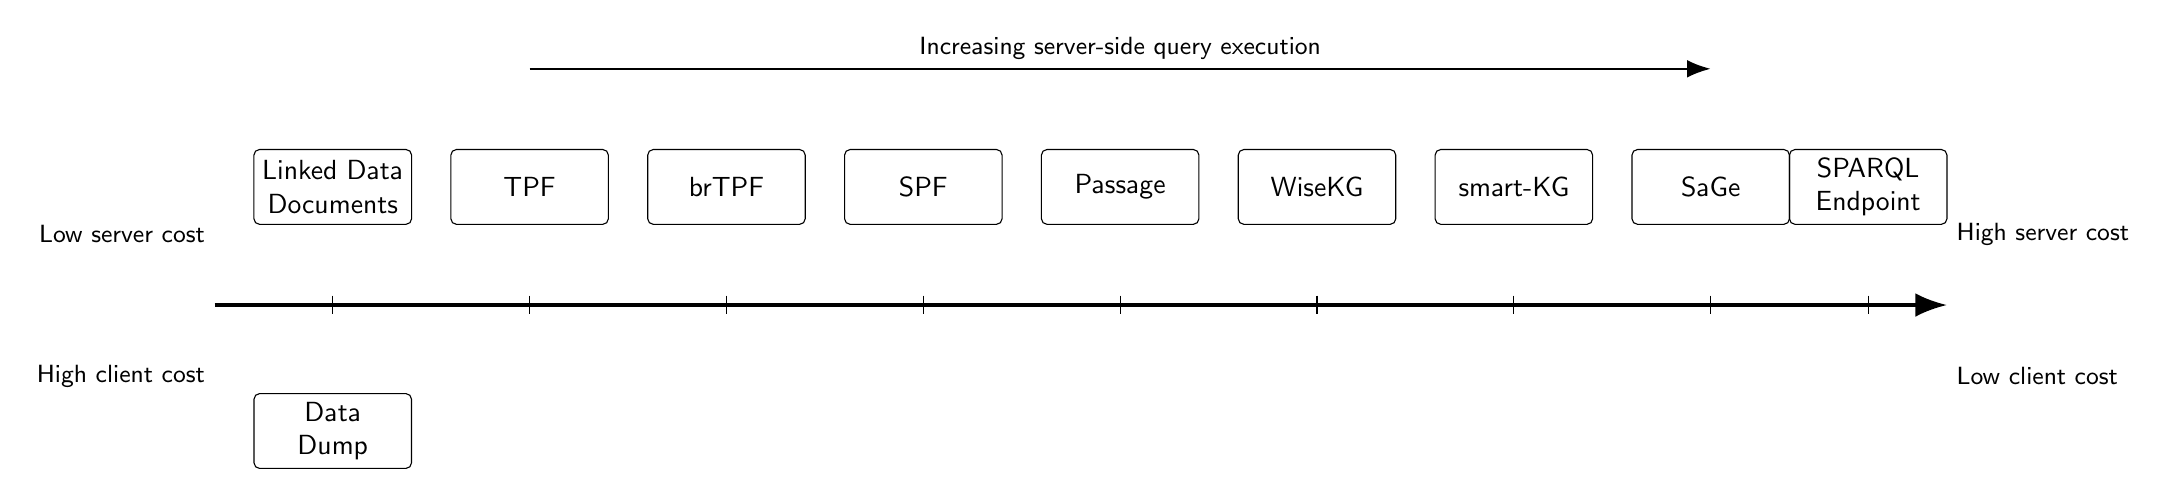
\begin{tikzpicture}[
    >=Latex,
    font=\sffamily,
    fragment/.style={
        draw,
        rounded corners=2pt,
        align=center,
        minimum width=2.0cm,
        minimum height=0.95cm,
        inner sep=3pt
    }
]

% --------------------------------------------------
% Axis
% --------------------------------------------------

\draw[very thick,-{Latex[length=4mm]}] (0,0) -- (22,0);

\node[anchor=east] at (0,0.9)
    {\small Low server cost};

\node[anchor=west] at (22,0.9)
    {\small High server cost};

\node[anchor=east] at (0,-0.9)
    {\small High client cost};

\node[anchor=west] at (22,-0.9)
    {\small Low client cost};

% --------------------------------------------------
% Tick marks
% --------------------------------------------------

\foreach \x in {1.5,4.0,6.5,9.0,11.5,14.0,16.5,19.0,21.0}
{
    \draw (\x,0.12) -- (\x,-0.12);
}

% --------------------------------------------------
% Main spectrum
% --------------------------------------------------

\node[fragment] at (1.5,1.5)
    {Linked Data\\Documents};

\node[fragment] at (4.0,1.5)
    {TPF};

\node[fragment] at (6.5,1.5)
    {brTPF};

\node[fragment] at (9.0,1.5)
    {SPF};

\node[fragment] at (11.5,1.5)
    {Passage};

\node[fragment] at (14.0,1.5)
    {WiseKG};

\node[fragment] at (16.5,1.5)
    {smart-KG};

\node[fragment] at (19.0,1.5)
    {SaGe};

\node[fragment] at (21.0,1.5)
    {SPARQL\\Endpoint};

% --------------------------------------------------
% Data dump
% --------------------------------------------------

\node[fragment] at (1.5,-1.6)
    {Data\\Dump};

% --------------------------------------------------
% Trend arrow
% --------------------------------------------------

\draw[thick,-{Latex[length=3mm]}]
    (4.0,3.0) -- (19.0,3.0);

\node[above] at (11.5,3.0)
    {\small Increasing server-side query execution};

\end{tikzpicture}

\end{document}